\documentclass[a4paper,11pt]{IEEEtran}
\hyphenation{op-tical net-works semi-conduc-tor}
\usepackage[pdftex]{graphicx}
\usepackage[scale=0.77,twoside,bindingoffset=5mm]{geometry}
\usepackage[onehalfspacing]{setspace}


\begin{document}
\title{Allergorithm}
\author{\IEEEauthorblockN{\small Han jeong u\\}
\IEEEauthorblockA{\small Information system\\
Hanyang university\\
seoul, korea\\
adfreeman@hanyang.ac.kr\\~\\}
\and
\IEEEauthorblockN{\small Lee su min\\}
\IEEEauthorblockA{\small Information system\\
Hanyang university\\
seoul, korea\\
qwer687@naver.com\\~\\}
\and
\IEEEauthorblockN{\small Lee si won\\}
\IEEEauthorblockA{\small Information system\\
Hanyang university\\
seoul, korea\\
trotism@naver.com}}
% make the title area
\maketitle
\begin{abstract}
%\boldmath
{\large}
{\large
Peoples are often eating allergic food such as milk,
bean, crab, eggs, peanuts ,cucumber and anything which have the possibility of causing allege reaction. Although people may want to have faith in food providers to provide good allergy protection, the confidentiality of any food in public can be violated, and consequently, while providers may not be “doing evil,” we can not and should not trust them with food confidentiality. we think that allergy protection technique is required. and also while the interest to allergy in society increase, The platform which comprehensively manage allergic is required. So, to better protect the confidentiality of school meal, We felt the need to develop Allergorithm, the system which mange allergic of elementary students. Allergorithm is a new approach to allergy confidentiality of elementary students that not only provides isolation from allergic foods but also preserves the students health through the creation of integrated management system of allergy. This approach allows Allergorithm to implement true end-to-end allergy protection of elementary students with three goals in mind: 1) isolation from allergic foods in school 2) quick SMS service to parents and teachers 3) easy-to-use interface. we were planning application which identify the student's allergy and provide an SMS service to teachers and parents in real-time. to do this, there are some need. first, allergic component should be numbered. Because it must be organized allergic factors. If you are allergic to components are not organized, it will be difficult in a scientific way to regularize. second, It should investigate the allergic status of elementary school students. Because it is the most basic materials. And it should extract information about the menu of the school. next, the menu should be compared with the data of allergic student. And a tool is needed to deliver the result to parents and teachers. And to exchange information between schools, or between schools and health centers will be able to make a better safety net of elementary school student. We would implement a prototype of Allergorithm and show that it can support a number of school system.
}
~\\
\end{abstract}

\IEEEpeerreviewmaketitle

\section{Introduction}
~\\
{\large
A continuously increasing number of elementary school student had eaten foods as an essential part of their daily lives. While many elementary schools are offering more and more meals to their students, the problem of food safety is unsolved. the default method of administrating them exposes students to Food risks, because it implicitly requires the students to trust the meal providers with the confidentiality of their food.  And no one would experience Allergy research for example, peanuts, eggs, wheat, peaches, crab foods with ingredients that cause allergies, etc., in elementary school. This situation can lead to fatal consequences. For example, in overseas because of accidental ingestion of peanut butter School children was dead by asphyxiation due to allergic reactions. Without considering these factors can lead to big accidents especially to children such as elementary students. And the United States in 2006, bill that foods that made by 8 Ingredients such as peanuts, milk, eggs, fish, shellfish, etc, causing the allergic should be displayed in easy and common language on food packaging was passed and has being implemented. However, despite the general industrial products have been displayed, school meals has not expressed an allergy. And even if it is displayed, it is difficult to recognize and mark a parent or teachers. And most of the schools, is not worrying about allergies due to a lot of work. As the damage is due to allergies, especially to the younger generation such as elementary school students occurs, the need to prevent these problems has increased. To alter this undesirable status quo, solutions should be built based on an updated trust model of everyday communication that better reflects the reality of the threats mentioned above. In particular, new solutions must first assume meal providers to be untrusted. This implies that all other entities that are controlled by the meal providers, including the allergic food that students ate, must also be assumed untrusted. Although there are a plethora of food available today, we observed that many of school meals provide allergic food.
}
~\\
\section{REQUIREMENT}
~\\
{\large
1. Important allergic number setting \\
2. elementary students allergic condition survey \\
3. Getting information from the school cafeteria menu\\
4. information database to store the ID, Password, information of students\\
5. Allergy number notation\\
6. Enter the critical allergy number database\\
7. Enter student information and menu information in the database\\
~\\
\begin{figure}[!h]
        \centering
        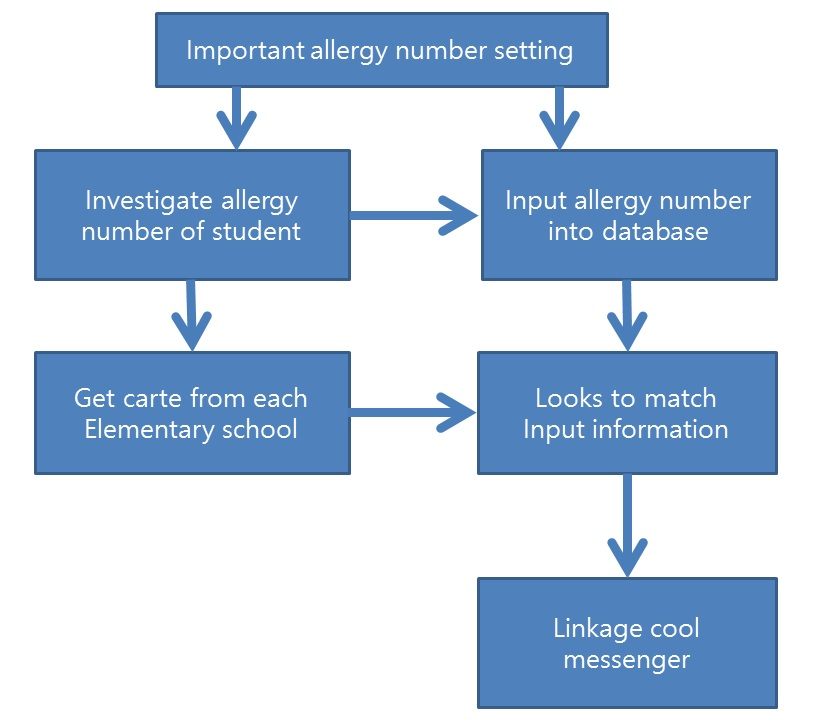
\includegraphics[width=0.5\textwidth, height=0.5\textheight]{s1.jpg}
        \caption{This figure is related to 1-7. First, important allergy number is set. And investigate the student and input allergy number to database. Second, get carte from each elementary school, and look to match the input information. Third, Send the analysed information to teachers through the cool messenger.}
        \label{fig1}
\end{figure}

8. Comparing two pieces of information (switch syntax used)\\
9. Teachers messenger programs (cool messenger)\\
10. the permission of interworking with a cool messenger   \\\
11. The specific method of delivering information to parents (SMS service)\\
~\\
\begin{figure}[!h]
        \centering
        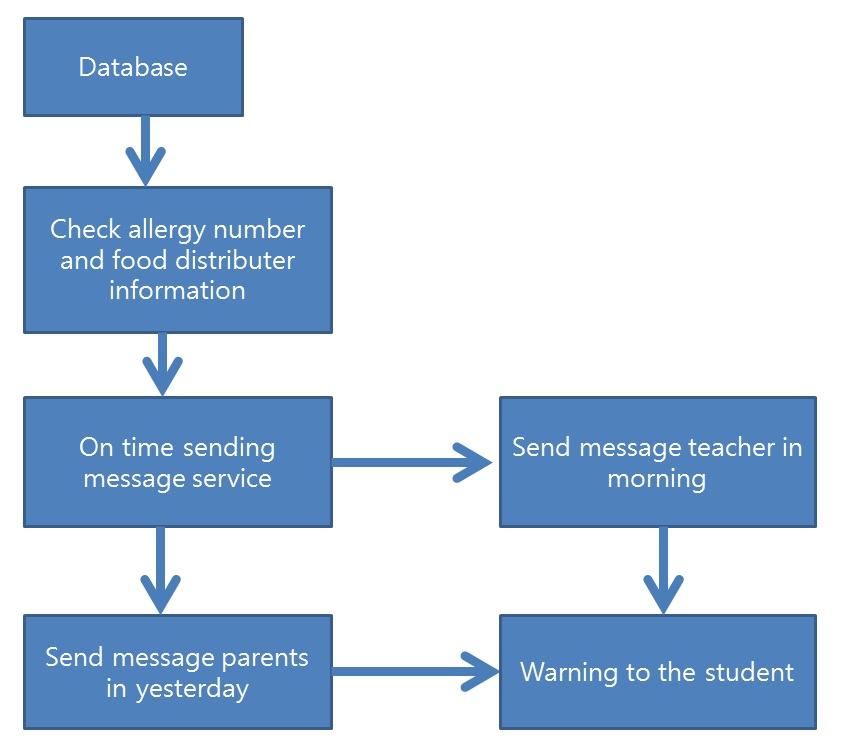
\includegraphics[width=0.5\textwidth, height=0.55\textheight]{s2.jpg}
        \caption{This figure is related to 8-11. Check the allergy number and food distributor information from database. And send message to parents and teacher. And at last warn to the student. }
        \label{fig1}
\end{figure}    
~\\
12. The program delivered to the teacher and parents (Need to distinguish code)\\
13. Checking that information has been forwarded to student\\
\clearpage
\begin{figure}[!h]
        \centering
        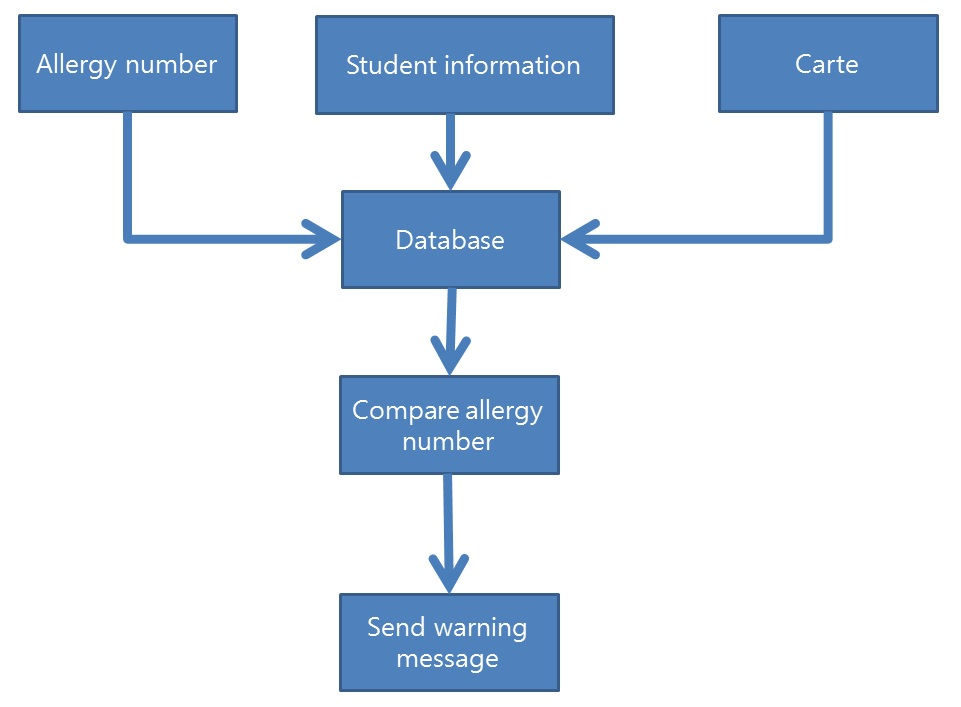
\includegraphics[width=0.5\textwidth, height=0.5\textheight]{s3.jpg}
        \caption{Input the allergy number, student information, carte to the database. In the program, Internal execution is executed by the switch statement. Selecting the internal message which have to send is executed by switch statement. And the information is conveyed to the message service.}
        \label{fig1}
\end{figure}
~\\
14. Allergic prevention education(parents perform allergy diagnostic tests instead of student Teachers carry out a direct tests)\\
15. Each school-based Interlocking System\\
16. In conjunction with the Department of Education or Health Center\\
~\\
\begin{figure}[!h]
        \centering
        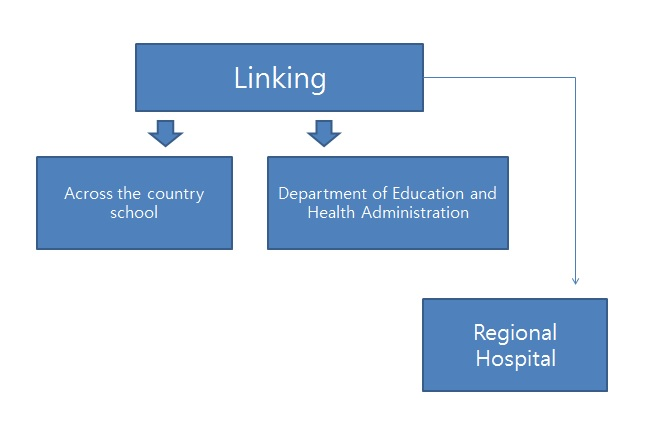
\includegraphics[width=0.5\textwidth, height=0.6\textheight]{s4.jpg}
        \caption{Link with the country school, department of education, health administration, and regional hospital.}
        \label{fig1}
\end{figure}
~\\
17. Cope ways after unexpected allergic damage happened due to the lack of information\\
18. after allergic damage occurs, first aid training (teacher)\\
19. allergic follow-up action after damage occurs (database update / furnishing the medicine)\\
~\\
\begin{figure}[!h]
        \centering
        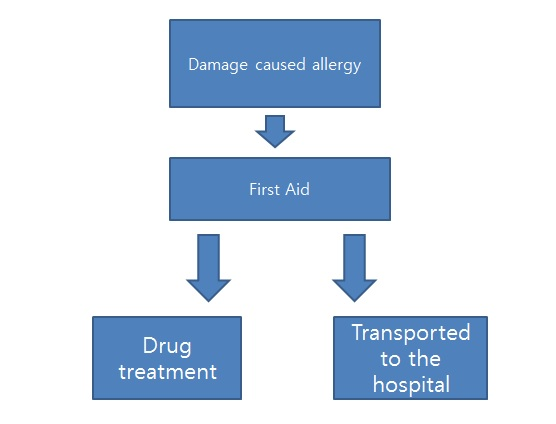
\includegraphics[width=0.5\textwidth, height=0.3\textheight]{s5.jpg}
        \caption{if damage caused by allergy is generated, the application inform that the emergency measures are necessary conditions to teachers. And application helps to evacuate injured student to hospital and put up the drug treatment. }
        \label{fig1}
\end{figure}
~\\
20. Alternative food preparation for Students who are experiencing allergies\\
21. If student can not eats meals, prepare lunch box or use near Shops.\\

\begin{figure}[!h]
        \centering
        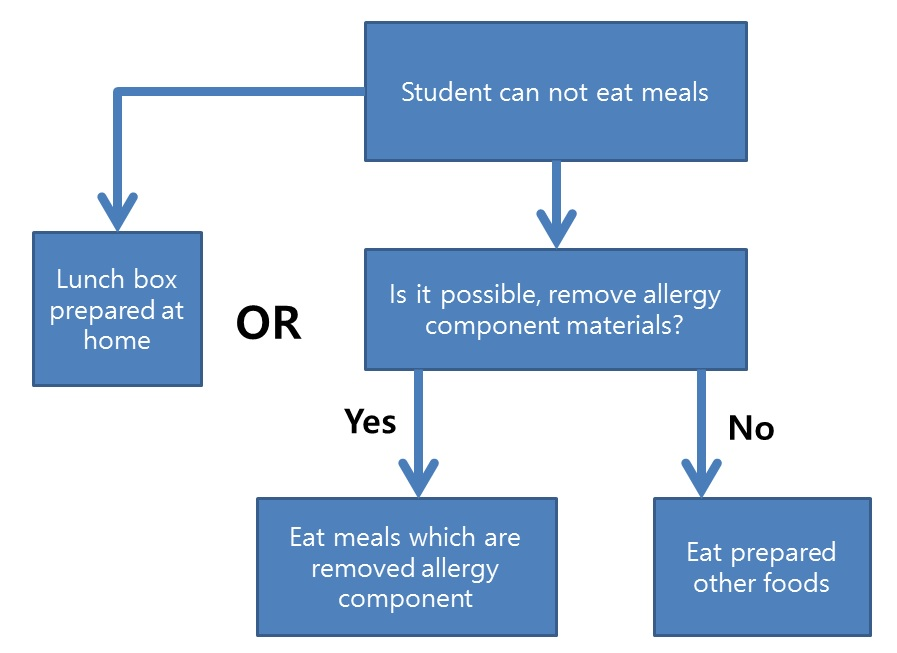
\includegraphics[width=0.5\textwidth, height=0.5\textheight]{s6.jpg}
        \caption{}
        \label{fig1}
\end{figure}
}
\newpage

\section{DEVELOPMENT ENVIRONMENT}
{\large
~\\
\section*{A. choice of software development platform}
~\\

Operating systems used primarily in elementary school is win-dows XP, 7, 8.1. Therefore, when testing a program is being developed, it may be appropriate to have a test in the Windows platform. And development environment for Windows is excellent. So we chose the windows platform. And we chose Java as a programming language. Because JAVA is an object-oriented language. Java has the following characteristics such of object orientation, language of safety, simplicity of language, and a wide range of standard library. So we chose  JAVA.
Development costs include operating costs cloud server, development tool (java, eclipse), sms service utilization costs.
Cloud server that use for database is amazon ec2 developer. 
This server is a cost of 49 dollar per month costs.
Development tool costs are zero because JAVA 1.8.0-31 version and Eclipse IDE for Java EE Developers SR2 win 64 bits are free software.
When developing SMS service, we wrote 10 cases for testing  based on NATE ON’s SMS service.
It took three hundred won.(1 case costs 30 won). Consider SMS service costs per school. Assume that each grade two hundred people per elementary school. An elementary school has one thousand two hundred students and has forty home room teacher(per thirty student). Sends SMS twenty days per month. Parent / home room teacher to send a text 20 * (1200 + 40) = 24800 counts should send a SMS. Nearly cost of 400,000 won based on ENPAX.
We will use the three laptop. 3 computers are all the windows 8.1. and JAVA version is 1. 8. 0-31. And software version is eclipse IDE for JAVA EE developers windows 64bit. Our computer’s specification is approximately ram 4G, intel i5 CPU, 120G ssd. We will use the amazon ec2 for database building and Q and A.
~\\
\section*{B. Software in use}
~\\
\begin{figure}[!h]
        \centering
        
\includegraphics[width=0.4\textwidth]{java.jpg}
        \caption{JAVA}
        \label{fig1}
\end{figure}
~\\
1.JAVA
~\\\\
key benefit of Java is its security features. Both the language and the platform were designed from the ground up with security in mind. The Java platform allows users to download untrusted code over a network and run it in a secure environment in which it cannot do any harm: it cannot infect the host system with a virus, cannot read or write files from the hard drive, and so forth. This capability alone makes the Java platform unique.
The Java 2 Platform takes the security model a step further. It makes security levels and restrictions highly configurable and extends them beyond applets. As of Java 1.2, any Java code, whether it is an applet, a servlet, a JavaBeans component, or a complete Java application, can be run with restricted permissions that prevent it from doing harm to the host system.
The security features of the Java language and platform have been subjected to intense scrutiny by security experts around the world. Security-related bugs, some of them potentially serious, have been found and promptly fixed. Because of the security promises Java makes, it is big news when a new security bug is found. Remember, however, that no other mainstream platform can make security guarantees nearly as strong as those Java makes. If Java's security is not yet perfect, it has been proven strong enough for practical day-to-day use and is certainly better than any of the alternatives.

Java is both dynamic and extensible. Java code is organized in modular object-oriented units called classes. Classes are stored in separate files and are loaded into the Java interpreter only when needed. This means that an application can decide as it is running what classes it needs and can load them when it needs them. It also means that a program can dynamically extend itself by loading the classes it needs to expand its functionality.
The network-centric design of the Java platform means that a Java application can dynamically extend itself by loading new classes over a network. An application that takes advantage of these features ceases to be a monolithic block of code. Instead, it becomes an interacting collection of independent software components. Thus, Java enables a powerful new metaphor of application design and development.
The Java language and the Java platform were designed from the start with the rest of the world in mind. Java is the only commonly used programming language that has internationalization features at its very core, rather than tacked on as an afterthought. While most programming languages use 8-bit characters that represent only the alphabets of English and Western European languages, Java uses 16-bit Unicode characters that represent the phonetic alphabets and ideographic character sets of the entire world. Java's internationalization features are not restricted to just low-level character representation, however. The features permeate the Java platform, making it easier to write internationalized programs with Java than it is with any other environment.
 Java programs are compiled to a portable intermediate form known as byte codes, rather than to native machine-language instructions. The Java Virtual Machine runs a Java program by interpreting these portable byte-code instructions. This architecture means that Java programs are faster than programs or scripts written in purely interpreted languages, but they are typically slower than C and C++ programs compiled to native machine language. Keep in mind, however, that although Java programs are compiled to byte code, not all of the Java platform is implemented with interpreted byte codes. For efficiency, computationally intensive portions of the Java platform--such as the string-manipulation methods--are implemented using native machine code.
Although early releases of Java suffered from performance problems, the speed of the Java VM has improved dramatically with each new release. The VM has been highly tuned and optimized in many significant ways. Furthermore, many implementations include a just-in-time compiler, which converts Java byte codes to native machine instructions on the fly. Using sophisticated JIT compilers, Java programs can execute at speeds comparable to the speeds of native C and C++ applications.
The final, and perhaps most important, reason to use Java is that We like it. Java is an elegant language combined with a powerful and well-designed set of APIs. Programmers enjoy programming in Java and are usually amazed at how quickly they can get results with it. Studies have consistently shown that switching to Java increases programmer efficiency. Because Java is a simple and elegant language with a well-designed, intuitive set of APIs, programmers write better code with fewer bugs than for other platforms, again reducing development time.
~\\
We had been looking for a software such as allergy management program, program related to allergy, and etc. but program like that isn’t exist. But algorithm Similar to what we are trying to implement is exist. Robot Vacuum Cleaner uses obstacle detection code.\\
~\\
2.mySQL
~\\
\begin{figure}[!h]
        \centering
        
\includegraphics[width=0.4\textwidth]{mysql.jpg}
        \caption{mySQL}
        \label{fig1}
\end{figure}
~\\
While a basic knowledge of SQL is required and most relational databases require the same knowledge MySQL is very easy to use. With only a few simple SQL statements, We can build and interact with MySQL. MySQL includes solid data security layers that protect sensitive data from intruders. Rights can be set to allow some or all privileges to individuals. Passwords are encrypted. MySQL is included for free with $NetWare® 6.5$ and available by free download from MySQL Web site. In the interest of speed, MySQL designers made the decision to offer fewer features than other major database competitors, such as $Sybase*$ and $Oracle*$. However, despite having fewer features than the other commercial database products, MySQL still offers all of the features required by most database developers. MySQL can handle almost any amount of data, up to as much as 50 million rows or more. The default file size limit is about 4 GB. However, it can increase this number to a theoretical limit of 8 TB of data. MySQL server has been thoroughly tested to prevent memory leaks. MySQL on NetWare runs effectively with $Novell®$ Cluster $Services™$. If one server goes down, MySQL on an alternate server takes over and customers won't know that anything happened. MySQL runs on many operating systems, including Novell NetWare, $Windows*$ $Linux*$, many varieties of $UNIX*$ (such as $Sun* Solaris*$, AIX, and $DEC* UNIX$), OS/2, $FreeBSD*$, and others. Development interfaces include JDBC, ODBC, and scripting (PHP and Perl), letting programmer create database solutions that run not only in NetWare 6.5 environment, but across all major platforms, including Linux, UNIX, and Windows.\\\\
~\\
3.window builder
~\\
\begin{figure}[!h]
        \centering
        
\includegraphics[width=0.4\textwidth]{windowbuilder.jpg}
        \caption{Window Builder}
        \label{fig1}
\end{figure}
~\\
WindowBuilder is composed of SWT Designer and Swing Designer and makes it very easy to create Java GUI applications without spending a lot of time writing code. Use the WYSIWYG visual designer and layout tools to create simple forms to complex windows; the Java code will be generated for you. Easily add controls using drag-and-drop, add event handlers to your controls, change various properties of controls using a property editor, internationalize your app and much more.
WindowBuilder is built as a plug-in to Eclipse and the various Eclipse-based IDEs (RAD, RSA, MyEclipse, JBuilder, etc.). The plug-in builds an abstract syntax tree (AST) to navigate the source code and uses GEF to display and manage the visual presentation.
Generated code doesn't require any additional custom libraries to compile and run: all of the generated code can be used without having WindowBuilder Pro installed. WindowBuilder Pro can read and write almost any format and reverse-engineer most hand-written Java GUI code. It also supports free-form code editing (make changes anywhere...not just in special areas) and most user re-factorings (you can move, rename and subdivide methods without a problem).
~\\
~\\~\\
4.eclipse
~\\
\begin{figure}[!h]
        \centering
        
\includegraphics[width=0.3\textwidth]{eclipse.jpg}
        \caption{Eclipse}
        \label{fig1}
\end{figure}
~\\
In computer programming, Eclipse is an integrated development environment (IDE). It contains a base workspaceand an extensible plug-in system for customizing the environment. Written mostly in Java, Eclipse can be used to develop applications. By means of various plug-ins, Eclipse may also be used to develop applications in other programming languages: Ada, ABAP, C, C++, COBOL, Fortran, Haskell,JavaScript, Lasso, Lua, Natural, Perl, PHP, Prolog, Python, R,Ruby (including Ruby on Rails framework), Scala, Clojure,Groovy, Scheme, and Erlang. It can also be used to develop packages for the software Mathematica. Development environments include the Eclipse Java development tools (JDT) for Java and Scala, Eclipse CDT for C/C++ and Eclipse PDT for PHP, among others.
The initial codebase originated from IBM VisualAge.[2] The Eclipse software development kit (SDK), which includes the Java development tools, is meant for Java developers. Users can extend its abilities by installing plug-ins written for the Eclipse Platform, such as development toolkits for other programming languages, and can write and contribute their own plug-in modules.
~\\
~\\
5.Jsmooth
~\\
~\\
\begin{figure}[!h]
        \centering
        
\includegraphics[width=0.4\textwidth]{jsmooth.jpg}
        \caption{Jsmooth}
        \label{fig1}
\end{figure}
~\\
JSmooth creates standard Windows executable files (.exe) that smartly launch java applications. It makes java deployment much smoother and user-friendly, as it is able to find and run Java VMs by itself, or help the user get one if none are available.\\
~\\
~\\
For example,\\
~\\
task main()
{  
  while(1)
  {
    int A=0, B=0, num;\\
    int total=0;\\
    nMotorEncoder[motorB] =0;\\
    nMotorEncoder[motorC] =0;\\
    motor[motorB] = 50;\\
    motor[motorC] = 50;\\
    wait1Msec(500);\\
  
    A = nMotorEncoder[motorB];\\
    B = nMotorEncoder[motorC];\\
    total = abs(B - A);\\
    while(total>4){\\
      num = random(2);\\
      motor[motorB] = 0;\\
      motor[motorC] = 0;\\
      wait1Msec(200);  \\
      if(num==0)\\
      {\\
        motor[motorB] = - 45;\\
        motor[motorC] = 45;\\
        wait1Msec(1000);\\
      }\\
      else\\
      {\\
        motor[motorB] = 45;\\
        motor[motorC] = -45;\\
        wait1Msec(1000);\\
      }\\
      total = 0;\\
      break;}\\
  }\\
}\\
\section*{C. Task distribution}
~\\
\begin{figure}[!h]
        \centering
        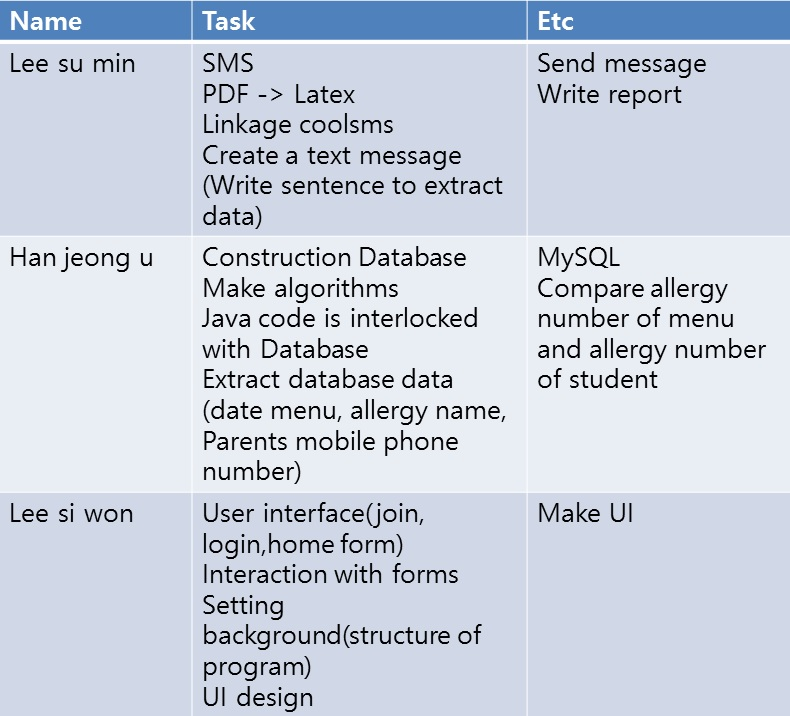
\includegraphics[width=0.55\textwidth, height=0.6\textheight]{ts.jpg}
        \caption{login window}
        \label{fig1}
\end{figure}
~\\
}
{\large
\section{SPECIFICATIONS}

\section*{A. requirement 1}
~\\

\begin{figure}[!h]
        \centering
        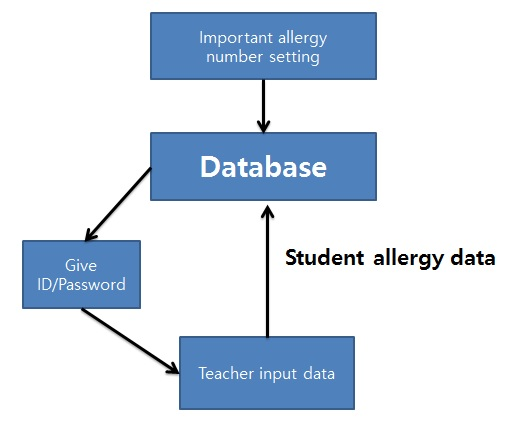
\includegraphics[width=0.5\textwidth, height=0.4\textheight]{r1.jpg}
        \caption{requirement1}
        \label{fig1}
\end{figure}

Gives a publicly available id / pw in each school. It should be implemented such as a direct generation, simultaneous access is possible, id / pw is based on the experience that you have saved in the DB and HTML makes it possible to work with JAVA for each school nutritionists. In this process, the session value, the id / pw should be able to match the DB. program will be get the login information from table teacher's info. and Value will be compared.
\section*{B. requirement 2}

\begin{figure}[!h]
        \centering
        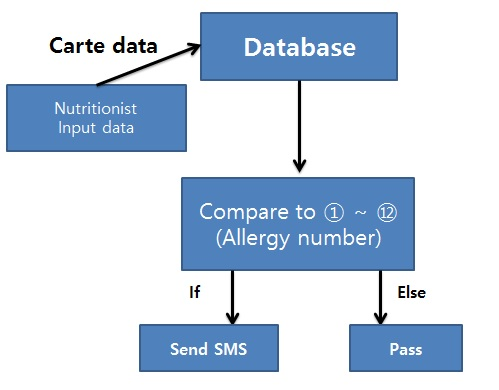
\includegraphics[width=0.5\textwidth, height=0.5\textheight]{r2.jpg}
        \caption{Caption}
        \label{fig1}
\end{figure}

There are menus in DB that can be registered dietitian. Elements of the submission form are weekday, date, and column.  column of the menu must be include feed materials name and allergic number Correspond-ing with feed materials. Allergy number is similar to most of the schools like a ①eggs, ② milk, ③ buckwheat, ④ peanuts, ⑤ soybean, ⑥ wheat, ⑦ mackerel, ⑧ it, ⑨ shrimp, ⑩ pork, ⑪ peach, ⑫ tomatoes. Therefore register that as a default value. Table that can be implemented a input, copy, paste. And Table can be matched with the allergy in DB, based on the value of the number entered in the (i, j).
For example (3, 2) there is a part in allergic value of 1,2,5,6,9,10 in alice elementary school lunch table.
~\\
\section*{C. requirement 3}
~\\
\begin{figure}[!h]
        \centering
        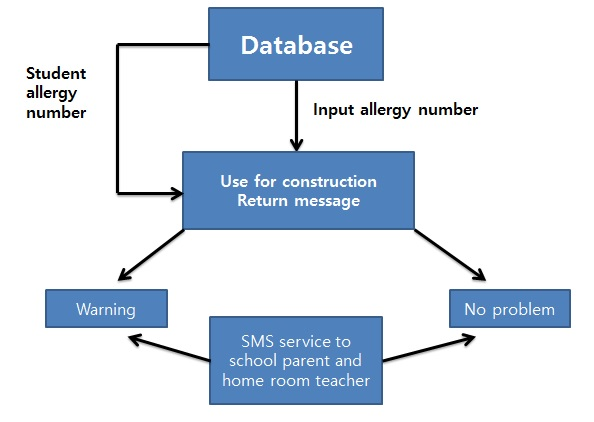
\includegraphics[width=0.5\textwidth, height=0.5\textheight]{r3.jpg}
        \caption{Caption}
        \label{fig1}
\end{figure}

The teacher should write the student's name, allergies number, parents 'names, parents' mobile phone number in the DB column. interlocking the feed table and the student table is important. For example, Suppose month 3, tuesday menu is Boiled barley and rice , Modern soup ⑤⑥, Pork jangjorim ①⑤⑥⑩, Kimchijeon ①⑤⑥⑨, Dices ⑨, milk ②. Set codes to run at 3/2 3pm. 
Search students with the value of 1,2,5,6,9,10, based on the student table comparing with allergy number of meals table. Briefly program code will work as follows by pseudocode.\\

for(int i=0; i< length; i++)\\
{ if(j==1 or 2 or 5 or 6 or 9 or 10) \\
return message(); // message method works.\\
}\\
SMS can be set to automatically transfer the student's parents. Run that code at am 7. Search student with the value of 1,2,5,6,9,10 interlocking with allergy number of meals table. Set the SMS to be sent automatically to home room teacher. To that Java and sms services should be linked.
~\\
}
{\large
\section{Architecture design and Implementation}
~\\
\section*{A. Overall architecture}
~\\
\begin{figure}[!h]
        \centering
        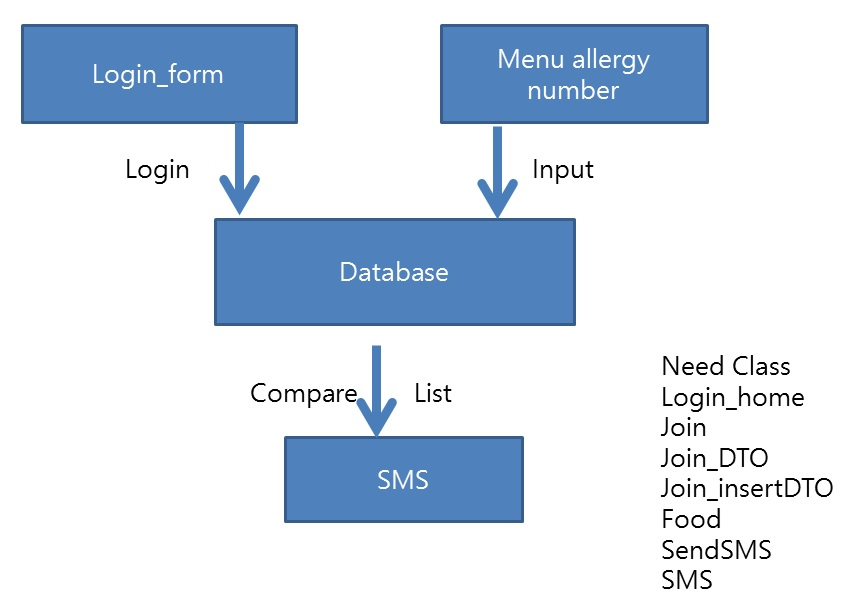
\includegraphics[width=0.5\textwidth, height=0.5\textheight]{oa1.jpg}
        \caption{overall architecture A}
        \label{fig1}
\end{figure}
~\\
Login and input data are necessary in order to enter data into the database. It must go through $login_form$ to login and it is necessary to input allergy number and menu into the database.After login and input data must be compared with each other in the database.Here, list which has been created to compare data is created. The list is a list of people to be send allergy warning letters. Required class are $Login_Home$, $Join$, $Join_DTO$, $Join_insertDTO$, $Food$, $SendSMS$ and $SMS$.
~\\
\begin{figure}[!h]
        \centering
        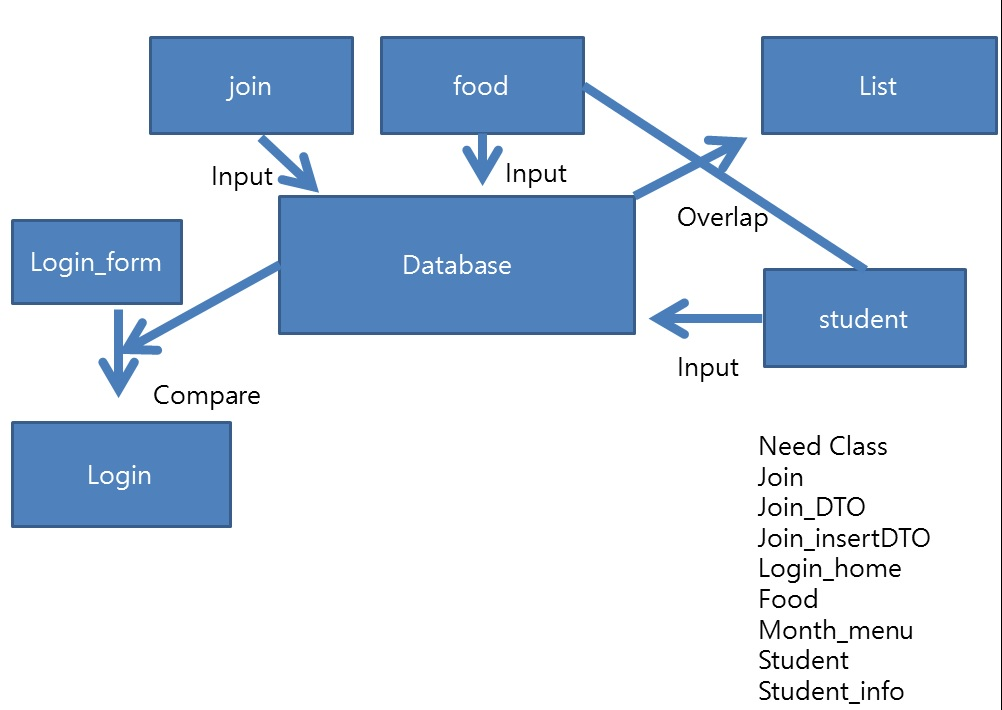
\includegraphics[width=0.5\textwidth, height=0.5\textheight]{oa2.jpg}
        \caption{overall architecture B}
        \label{fig1}
\end{figure}
~\\
This figure 16 is a figure that describes in more detail about login and input data. Login must be a priority sign up at Join. Sign up data goes into the database. When you login in $login_form$, compares join data and login data. After login, enter menu through food class and enter student data through $student_info$ class. Next, compared to menu and student data to create a list. Required class are $Login_Home$, Join, $Join_DTO$, $Join_insertDTO$, Food, Month menu, Student and $Student_info$.\\
In order to login should be matched entered id / pw and id / pw in datebase. Process to achieve login is through the following code.
~\\
\\
void loginCheck() {\\
id = $in_id$.getText().trim();\\
pw = $in_pw$.getText().trim();\\
~\\
String query = "SELECT pw,name FROM $teacher_info$ where id='" + id + "'"\\
~\\
System.out.println(query);\\
try{\\
ResultSet rs = stmt.executeQuery(query);\\
\\\\
if (rs.next()) {\\
name = rs.getString("name");\\
~\\
if (pw.equals(rs.getString("pw"))) {
~\\
   System.out.println("확인되었습니다.");\\
   home frame = new home();\\
   frame.setVisible(true);\\
}\\\\
~\\
After id/pw come take by getText, through string query receives id / pw in the database. Next, use if sentence. If id/pw match, goes menu input / student information input form. Information is entered in menu input form is sent to database by following code.(date, three allergy component in menu)
~\\~\\
JLabel lname = new JLabel("date");\\
lname.setBounds(17, 58, 78, 21);\\
p.add(lname);\\
~\\
$in_Pname$ = new JTextField();\\
$in_Pname$.setBounds(153, 123, 156, 27);\\
p.add($in_Pname$);\\
$in_Pname$.setColumns(10);\\
~\\
JLabel lpname = new JLabel("allergy number1");\\
lpname.setBounds(17, 126, 102, 21);\\
p.add(lpname);
~\\
$all_num1$ = new JTextField();\\
$all_num1$.setBounds(153, 192, 156, 27);\\
p.add($all_num1$);\\
$all_num1$.setColumns(10);\\
~\\
JLabel lblAllergyNumber = new JLabel("allergy number2");\\
lblAllergyNumber.setBounds(17, 195, 129, 21);\\
p.add(lblAllergyNumber);\\
~\\
$all_num2$ = new JTextField();\\
$all_num2$.setBounds(153, 265, 156, 27);\\
p.add($all_num2$);\\
$all_num2$.setColumns(10);\\
~\\
JLabel $lblAllergyNumber_1$ = new JLabel("allergy number3");\\
$lblAllergyNumber_1$.setBounds(17, 268, 129, 21);\\
p.add($lblAllergyNumber_1$);\\
~\\
Student information is sent to database by following code. (name, parent name, parent mobile, teacher name, teacher mobile must be entered and school name allergy numbers of students are not need to register.)
~\\
JLabel lname = new JLabel("name");\\
lname.setBounds(17, 58, 78, 21);\\
p.add(lname);\\
~\\
$in_Pname$ = new JTextField();\\
$in_Pname$.setBounds(153, 100, 156, 27);\\
p.add($in_Pname$);\\
$in_Pname$.setColumns(10);\\
~\\
JLabel lpname = new JLabel("parent name");\\
lpname.setBounds(17, 103, 102, 21);\\
p.add(lpname);\\
~\\
$in_Pmobile$ = new JTextField();\\
$in_Pmobile$.setBounds(153, 142, 156, 27);\\
p.add($in_Pmobile$);\\
$in_Pmobile$.setColumns(10);\\
~\\
JLabel lblParentMobile = new JLabel("parent mobile");\\
lblParentMobile.setBounds(17, 145, 109, 21);\\
p.add(lblParentMobile);\\
~\\
$in_Tname$ = new JTextField();\\
$in_Tname$.setBounds(153, 184, 156, 27);\\
p.add($in_Tname$);\\
$in_Tname$.setColumns(10);\\
~\\
JLabel lblTeacherName = new JLabel("teacher name");\\
lblTeacherName.setBounds(17, 187, 112, 21);\\
p.add(lblTeacherName);\\
~\\
$in_Tmobile$ = new JTextField();\\
$in_Tmobile$.setBounds(153, 226, 156, 27);\\
p.add($in_Tmobile$);\\
$in_Tmobile$.setColumns(10);\\
~\\
JLabel lblTeacherMobile = new JLabel("teacher mobile");\\
lblTeacherMobile.setBounds(17, 229, 119, 21);\\
p.add(lblTeacherMobile);\\
~\\
$in_Sname$ = new JTextField();\\
$in_Sname$.setBounds(153, 268, 156, 27);\\
p.add($in_Sname$);\\
$in_Sname$.setColumns(10);\\
~\\
JLabel lblSchoolName = new JLabel("school name");\\
lblSchoolName.setBounds(17, 271, 106, 21);\\
p.add(lblSchoolName);\\
~\\
$all_num1$ = new JTextField();\\
$all_num1$.setBounds(153, 310, 156, 27);\\
p.add($all_num1$);\\
$all_num1$.setColumns(10);\\
~\\
JLabel lblAllergyNumber = new JLabel("allergy number1");\\
lblAllergyNumber.setBounds(17, 313, 129, 21);\\
p.add(lblAllergyNumber);\\
~\\
$all_num2$ = new JTextField();\\
$all_num2$.setBounds(153, 352, 156, 27);\\
p.add($all_num2$);\\
$all_num2$.setColumns(10);\\
~\\
JLabel $lblAllergyNumber_1$ = new JLabel("allergy number2");\\
$lblAllergyNumber_1$.setBounds(17, 355, 129, 21);\\
p.add($lblAllergyNumber_1$);\\\\
You have entered all of monthly menu / student information in the database.
~\\
 int day = gc.get(Calendar.DATE);\\
~\\
Through the above code, come take a date. Next, Call today menu.\\
~\\
while (rs.next()) {
$stu_an1$ = Integer.parseInt(rs.getString("$allerg\\y_num1$"));\\
$stu_an2$ = Integer.parseInt(rs.getString("$allerg\\y_num2$"));\\
$stu_an3$ = Integer.parseInt(rs.getString("$allerg\\y_num3$"));\\
}\\
~\\
Through the above code, It brings menu allergy numbers.
\newpage
\begin{figure}[!h]
        \centering
        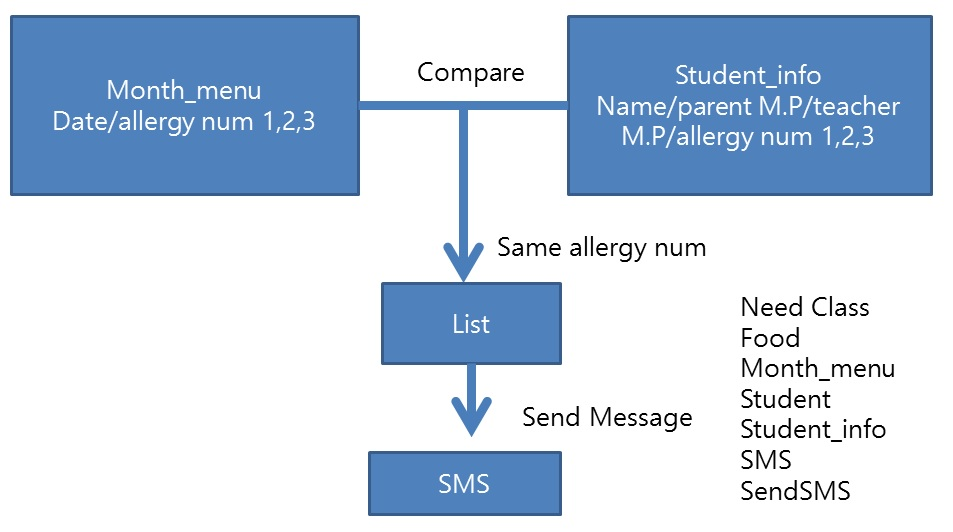
\includegraphics[width=0.5\textwidth, height=0.5\textheight]{oa3.jpg}
        \caption{Caption}
        \label{fig1}
\end{figure}
~\\
This figure is a figure that describes in more detail about compare to menu data and student data. Enter date menu and allergic number in Month menu class. Enter student name, parent mobile phone number, teacher mobile phone number and allergy number of student in $Student_info$ class. And compare the menu allergy number and student allergy number to look for same allergy number. Make a list that is made up students who has same allergy number.Information on the list of students send in SendSMS class.

Required class are Food, Month menu, Student, $Student_info$, SMS and SendSMS.\\
~\\
From now on allergy number of menu and allergy number of students, show how to send a text to match students.

for(int i=1; i<3; i++)
{
getAlnum(i);
if($stu_an1$ == td.$stu_an1$\\ 
$||$ $stu_an1$ == td.$stu_an2$\\
$||$ $stu_an1$ == td.$stu_an3$)\\
$result_an1$ = $stu_an1$\\
else\\
$result_an1$ = 0;\\
if($stu_an2$ == td.$stu_an1$\\ 
$||$ $stu_an2$ == td.$stu_an2$ \\
$||$ $stu_an2$ == td.$stu_an3$)\\
$result_an2$ = $stu_an2$\\
else\\
$result_an2$ = 0;\\
if($result_an1$ != 0 \\
$||$ $result_an2$ != 0 )\\
textSend($result_an1$, $result_an2$, $parent_phone$);\\
}\\
}
~\\
Above code confirms whether match allergy numbers of menu and allergy numbers of student. And Information of match student brings allergy numbers, parents mobile phone number in below code.

void getAlnum (int i) throws SQLException\\
{\\
String r1 = null,r2 = null\\
DbCon();\\
String query = "SELECT name, $allergy_num1$, $allergy_num2$,\\ $parent_phone$ FROM $student_info$ where no='"+i+"'"\\
ResultSet rs = stmt.executeQuery(query);\\
\\
while (rs.next()) {\\
r1 = rs.getString("$allergy_num1$");\\
r2 = rs.getString("$allergy_num2$");\\
$parent_phone$ = rs.getString("$parent_phone$");\\
}\\

if(!(r1.equals(null)))\\
$stu_an1$ = Integer.parseInt(r1);\\
else\\
$stu_an1$ = 0;\\

if(!(r2.equals(null)))\\
$stu_an2$ = Integer.parseInt(r2);\\
else\\
$stu_an2$ = 0;\\
}\\
And use following code so as to send a warning message.\\
\\
SMS sms = new SMS();\\
        sms.appversion("TEST/1.0");\\
        sms.charset("utf8");\\
        sms.setuser("coolsms id", “coolsms password”);\\
\\
        SmsMessagePdu pdu = new SmsMessagePdu();\\
        pdu.type = "SMS"\\
        pdu.destinationAddress = pp\\
        pdu.scAddress = "01044878704"\\
        pdu.text = "내일 급식에 "+r1+"성분과 "+r2+"성분이 있으니 주의하십시오."\\
        sms.add(pdu);\\\\

After link coolsms so as to send the character, make parent mobile phone number is pp, allergy components r1, r2 and write warning message.
For reference, process of converting a allergy number to allergy name is as follows.\\\\

aln = new String[12];\\
\\
aln[0]= "난류"\\
aln[1]= "우유"\\
aln[2]= "밀"\\
aln[3]= "보리"\\
aln[4]= "옥수수"\\
aln[5]= "쌀"\\
aln[6]= "메밀"\\
aln[7]= "땅콩"\\
aln[8]= "대두콩"\\
aln[9]= "새우"\\
aln[10]= "토마토"\\
aln[11]= "돼지고기"\\
\\
for(int i=1; i<13; i++)\\
{\\
if(r1 == i)\\
s1 = new String(aln[i-1]);\\
}\\
\\
for(int i=1; i<13; i++)\\
{\\
if(r2 == i)\\
s2 = new String(aln[i-1]);\\
}\\
\begin{figure}[!h]
        \centering
        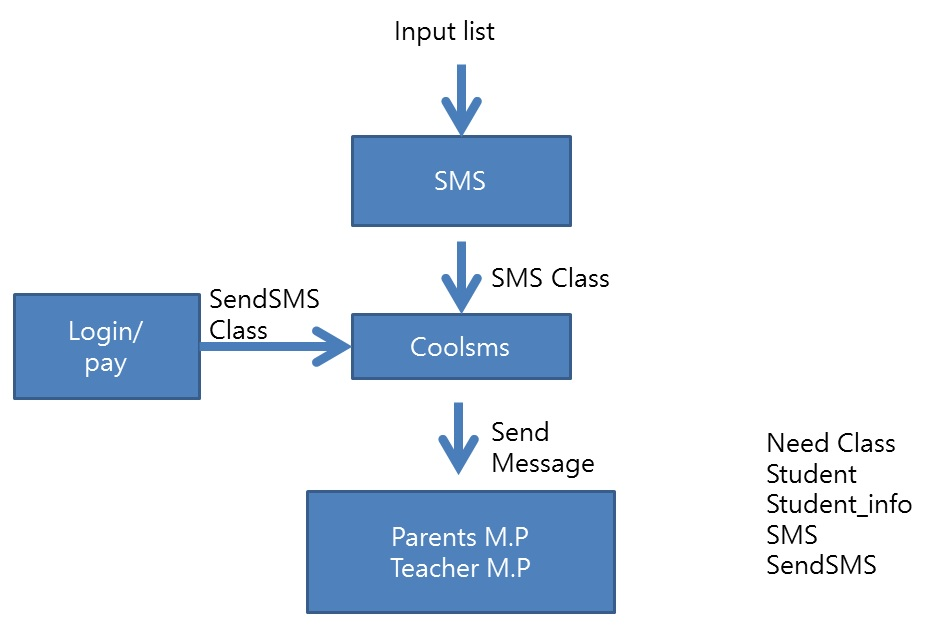
\includegraphics[width=0.5\textwidth, height=0.5\textheight]{oa4.jpg}
        \caption{figure 19}
        \label{fig1}
\end{figure}
~\\
This figure 19 describes in more detail about sendSMS. Receive a list of Students from list. In order to send sms, coolsms that site is provide short message service linked inSMS class. Beforehand enter recipient, caller information, originating time, and coolsms login data in SendSMS class. Bring to parents mobile phone number andteachers mobile phone number in $student_info$ class. It sends allergy warning letters to each mobile phone number go through SendSMS class.Required class are Student, $Student_info$, SMS and SendSMS. class student is form of receiving information and deliver the information to sendSMS. sendSMs generates the object of SMS. After passing the parent phone number, the object of sms has received the information.
~\\
\section*{B. Directory organization}
~\\
\begin{figure}[!h]
        \centering
        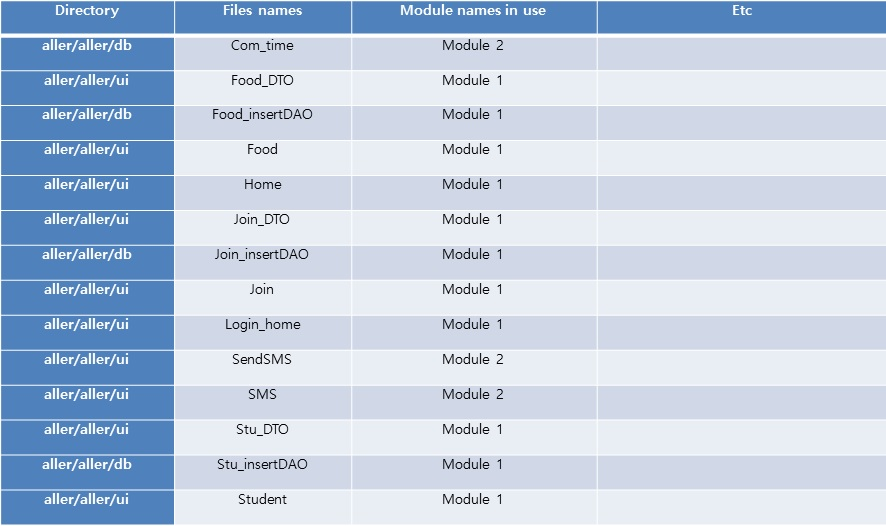
\includegraphics[width=0.5\textwidth, height=0.5\textheight]{do.jpg}
        \caption{Directory organization}
        \label{fig1}
\end{figure}
~\\
\section*{C. Module 1 or Software Component 1 or Class Name 1}
~\\
\begin{figure}[!h]
        \centering
        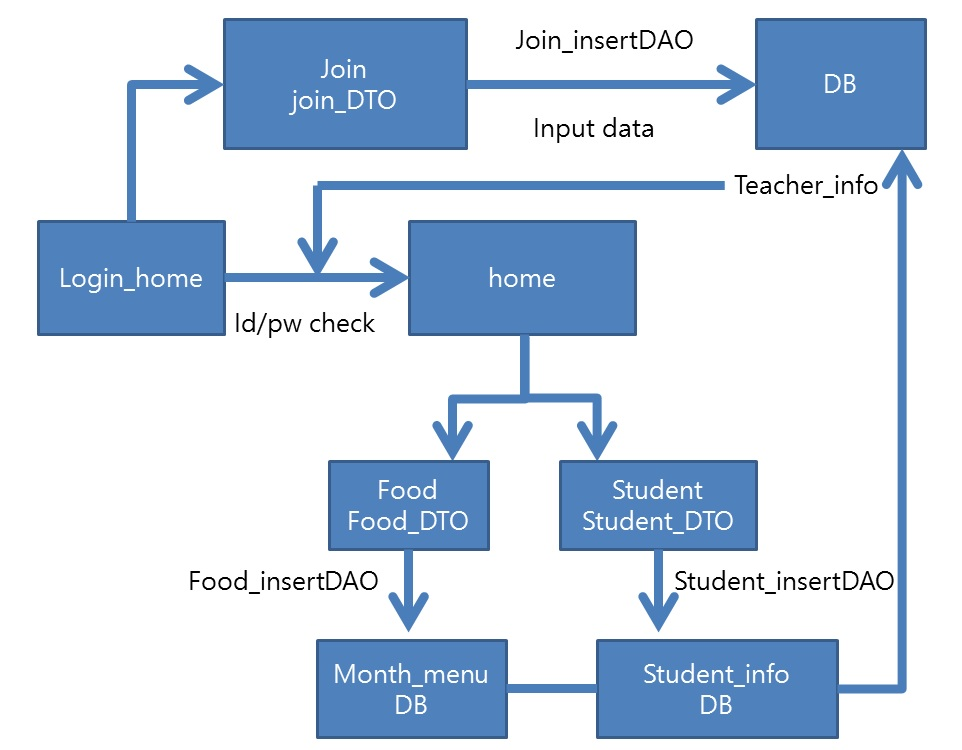
\includegraphics[width=0.5\textwidth, height=0.5\textheight]{m1.jpg}
        \caption{figure 21}
        \label{fig1}
\end{figure}
Module 1 is operated in accordance with five kinds of order. First, input data relating to teacher through join and stores data in the database.
Second,Id / pw through login and id / pw in database are to make sure it matches.
Third, Enter carte and student information and then stored in a database.
Fourth, Extract date menu's allergy information in $Month_menu$.
Last. Extract student's allergy information in $student_info$.

On the top join, $join_DTO$, $join_insertDAO$ are located. Should be entered the registration information(id/pw) at join and save information at $join_DTO$ and enter information into database at $join_insertDAO$. There are home and $login_home$ at the bottom. Enter your id / pw required to log in $login_home$. Confirm entered in $login_home$ id / pw exactly matches entered at the join and stored in the database id / pw.If you do not match, Pop up login failed. After a successful login, you can enter carte and student information. Carte-related information is sent to food student-related information is sent to student. Each of the entered data is stored in the $food_DTO$ and $student_DTO$.Sends to data in database through $food_insertDAO$ and $student_insertDAO$. Food-related database is $month_menu$ and student-related database is $student_info$.
~\\
\section*{D. Module 2 or Software Component 2 or Class Name 2}
~\\
\begin{figure}[!h]
        \centering
        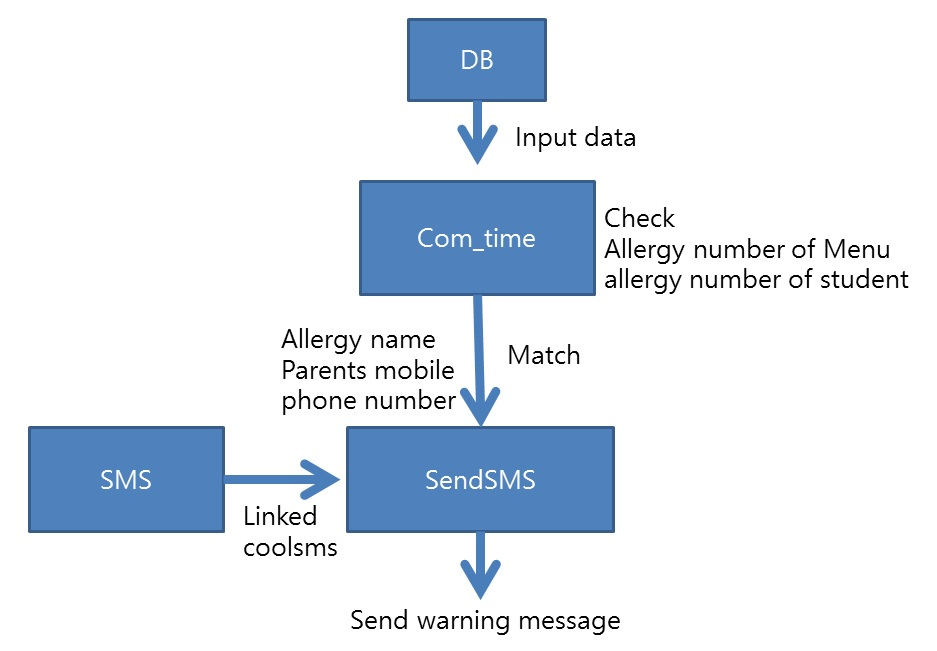
\includegraphics[width=0.5\textwidth, height=0.5\textheight]{m2.jpg}
        \caption{figure 22}
        \label{fig1}
\end{figure}
~\\
Module 2 is operated in accordance with four kinds of order.
First, Compare allergy number of date menu and allergy number of students $Com_time$.
Second, Extract student who matched allergy number parent's mobile phone number and allergy name.
Third, Create a small sentence allergy name that contains tomorrow menu  in SendSMS.
Last, Transmits warning message to the parent's mobile phone number.

Confirm allergy number of food stored in the module 1 exactly matches allergy number of student stored in the module 1 in $Com_time$.If allergy number matched, extract allergy names and phone numbers of the parents of the students. If it does not match, examine the following students.Parents mobile phone numbers are taken from $student_info$ in module 1. And allergy names are taken from $Com_time$ from in module 2.Using the above two kinds of information, create a warning message which contain sentence "Tomorrow at lunch allergy names components, so be careful" to parents mobile phone number through SendSMS.Next, Through liked coolsms in SMS, transfer the warning message written by SendSMS to parents mobile phone number.
~\\
~\\
}
{\large
\section{Use cases}
~\\
\section*{A. Use case 1}
~\\

\begin{figure}[!h]
        \centering
        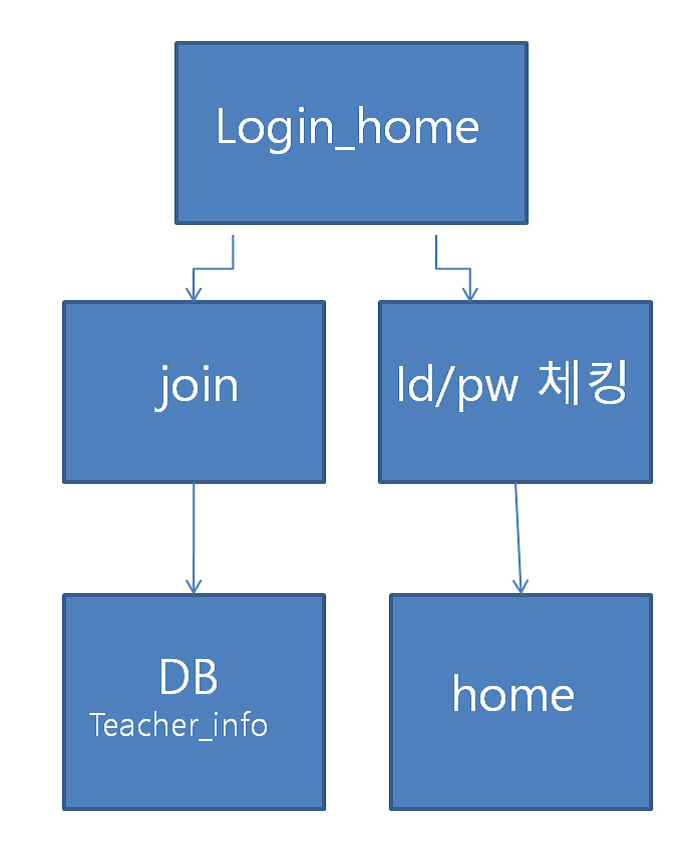
\includegraphics[width=0.5\textwidth, height=0.5\textheight]{usec1.jpg}
        \caption{}
        \label{fig1}
\end{figure}
~\\
this figure 23 shows join and login algorithm. if you click the "join" button and Fill out the form, your information will be entered to table $teacher_info$. and if you click the "login" button and fill out the form, program should be reading the login information in the table $teacher_info$. and If the values match, user will see the home screen.
~\\
\begin{figure}[!h]
        \centering
        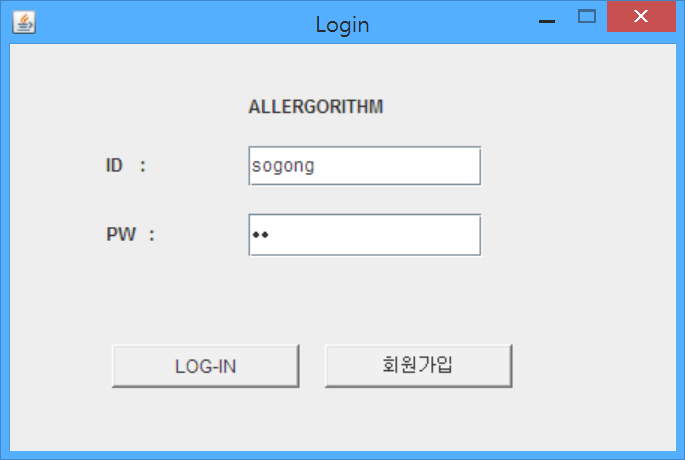
\includegraphics[width=0.4\textwidth]{usec2.jpg}
        \caption{}
        \label{fig1}
\end{figure}
~\\
discuss about login and join mechanism in figure 24. id and pw are identification number and password. you can see ”log-in” and ”Sign Up” button. first, user(teacher) click ”Sign Up” button on Bottom right. user will see the registration window such as figure 18. The user write the information into the compartment such as id, pw, name, mobile, phone. and if user click ”sign up” button ,information should go into the table teacherinfoof database allergorithm. and window of join should shut down. This is possible because the login information of the user now been stored in the database. when the user enter id and password in the text field and click on the ”log-in” button, id and password value of the user shall be checked whether valid. if the value of id and password is valid, home panel pop up. If you write ID/Password, the login program search the databases. If ID/Password are wrong like the above figure. It cannot get next step. 
~\\
\begin{figure}[!h]
        \centering
        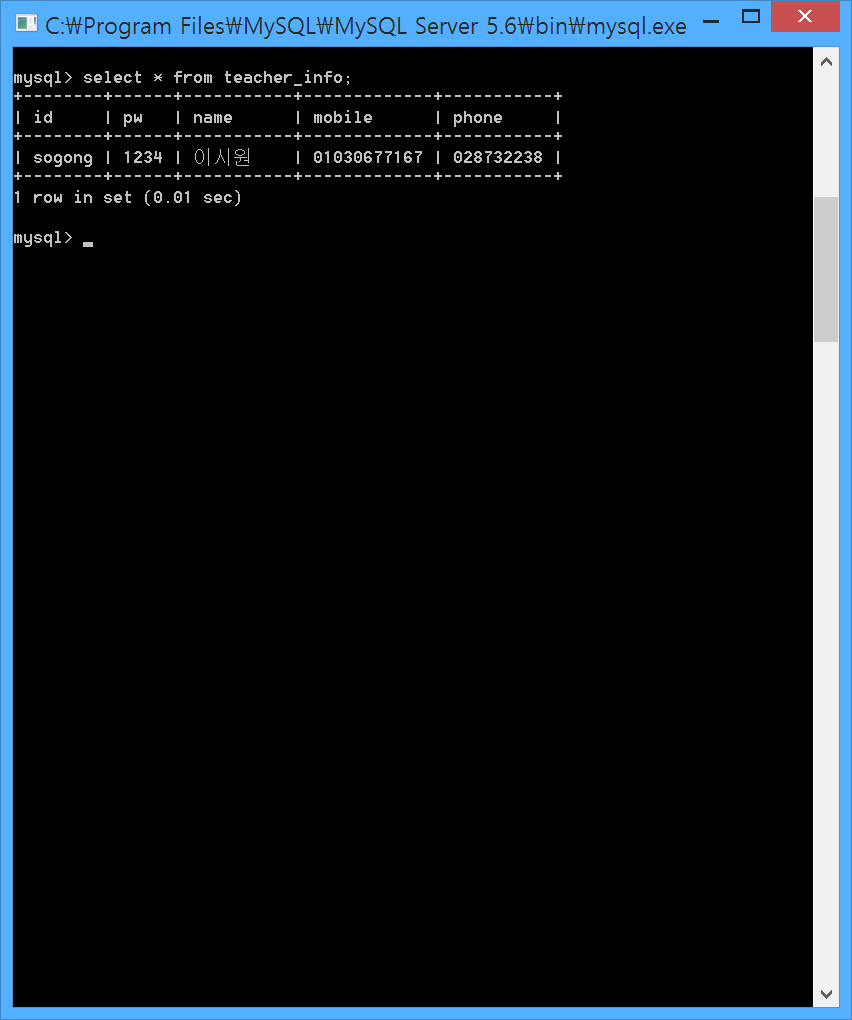
\includegraphics[width=0.5\textwidth, height=0.37\textheight]{usec3.jpg}
        \caption{}
        \label{fig1}
\end{figure}
~\\
The figure 25 is the database that contain the information about teacher. We create 3 tables which are $teacher_info$, $student_info$, $month_menu$. $Teacher_info$ has teacher's ID/Password/name/mobile/phone number. This table is needed for the login. If you write ID and password at the login form, the program will match it with this $teacher_info$ table. The ID is sogong but the Password is wrong. So It will be error. Then, Let’s click the join button. And go to the join form.
~\\
\begin{figure}[!h]
        \centering
        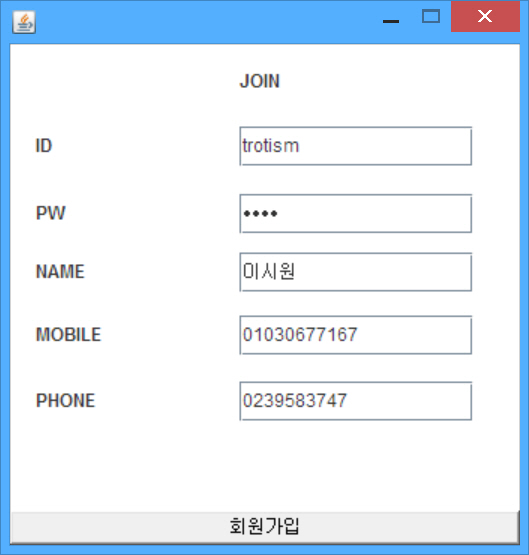
\includegraphics[width=0.4\textwidth]{usec4.jpg}
        \caption{}
        \label{fig1}
\end{figure}
~\\
Sign Up button is pressed, the screen will pop up, such as the above photo. Need to enter information are name, parent name, parent mobile phone number, teacher name, teacher mobile phone number, school name, two kinds of allergy numbers that student has allergy. Two kinds of allergy numbers are not mandatory, but the rest is essential. If enter all of the information and press save button, information are sent to the database. Name, parent name, parent mobile phone number, two kinds of allergy numbers move to student. Next information save on $student_DTO$ and are prepared to send to the database. Finally information sends the information to a database in $student_insertDAO$ and save on $student_info$. teacher name, teacher mobile phone number move to teacher. Next information save on $teacher_DTO$ and are prepared to send to the database. Finally information sends the information to a database in $teacher_insertDAO$ and save on $teacher_info$.
~\\
\begin{figure}[!h]
        \centering
        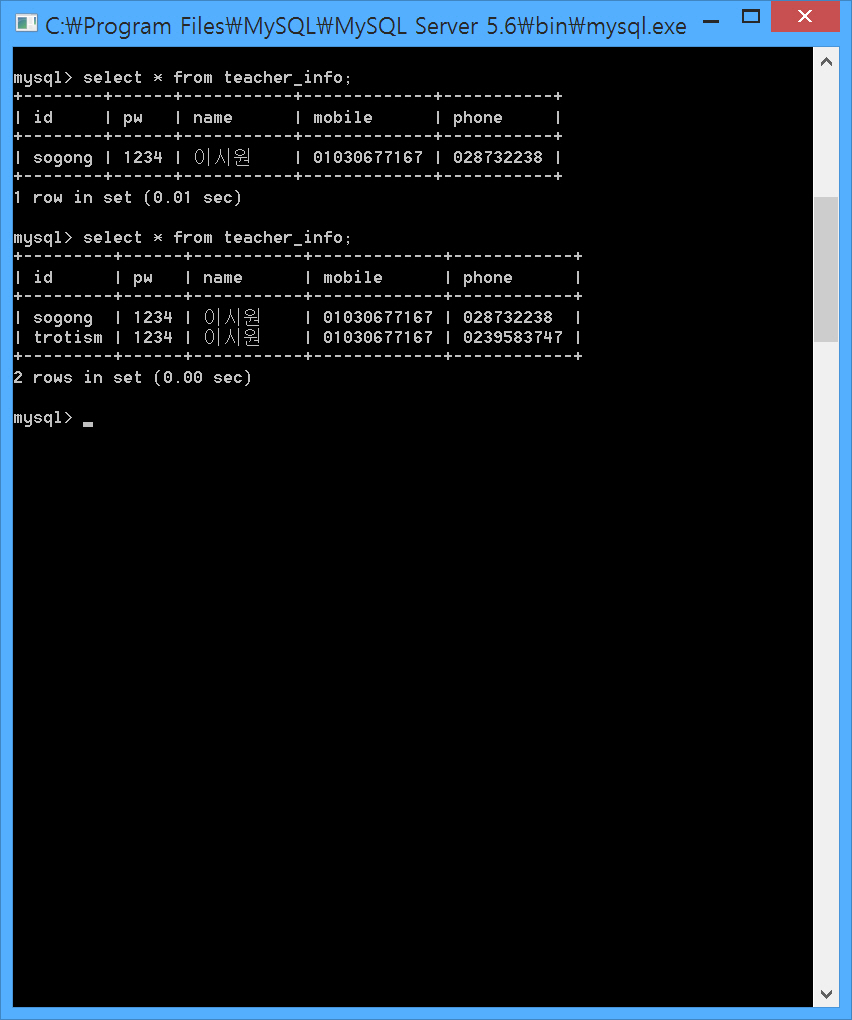
\includegraphics[width=0.5\textwidth, height=0.5\textheight]{usec5.jpg}
        \caption{}
        \label{fig1}
\end{figure}
~\\
~\\
\newpage
\begin{figure}[!h]
        \centering
        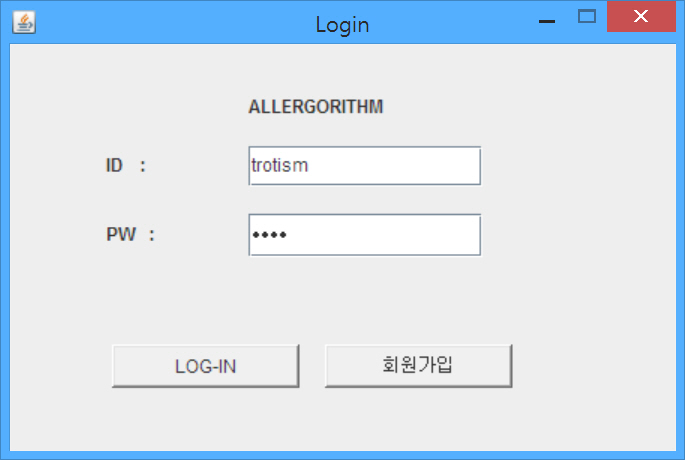
\includegraphics[width=0.4\textwidth]{usec6.jpg}
        \caption{}
        \label{fig1}
\end{figure}
~\\
Because you write the information and click the join button, It is executed, and this is the result. At the figure 25, $teacher_info$ table has only one ID:sogong. After the join, there is one more information whose ID is trotism. ID/Password/name/mobile/phone information are stored in the database.
~\\
\begin{figure}[!h]
        \centering
        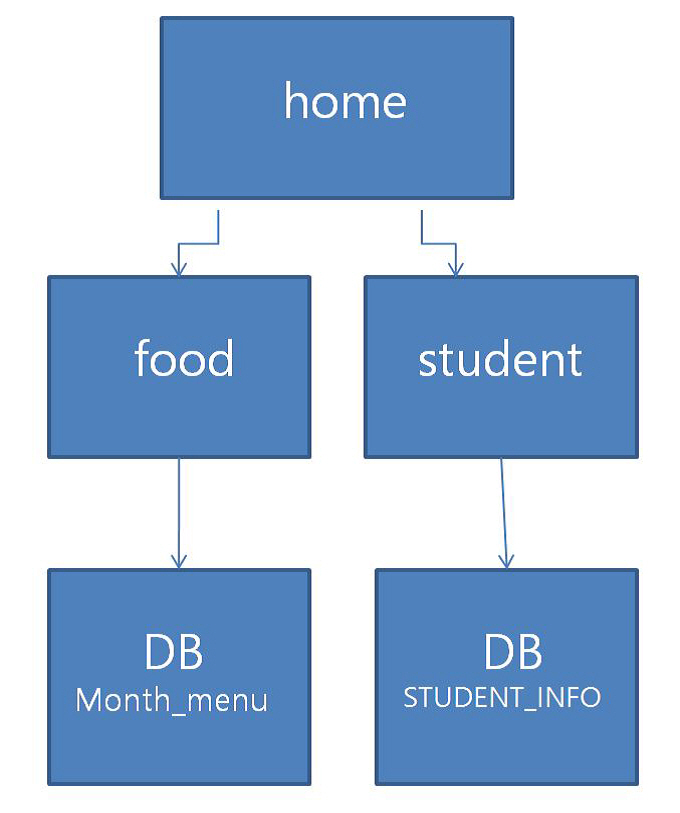
\includegraphics[width=0.5\textwidth, height=0.4\textheight]{usec7.jpg}
        \caption{}
        \label{fig1}
\end{figure}
~\\
Then, if you write the correct ID/Password, you can get the Home form.
~\\
\begin{figure}[!h]
        \centering
        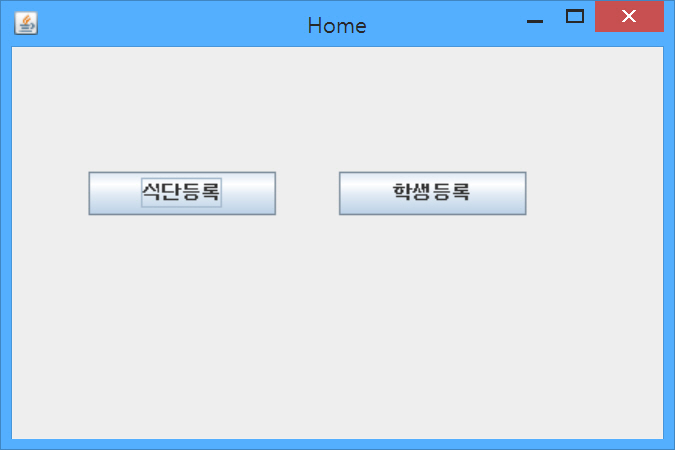
\includegraphics[width=0.4\textwidth]{usec8.jpg}
        \caption{}
        \label{fig1}
\end{figure}
~\\
The left side button is food register button for the food manager, and the right side button is student register button for the teacher who take care of their students. 
First, if you press the right button that can register the student information this figure pops out.
~\\
\begin{figure}[!h]
        \centering
        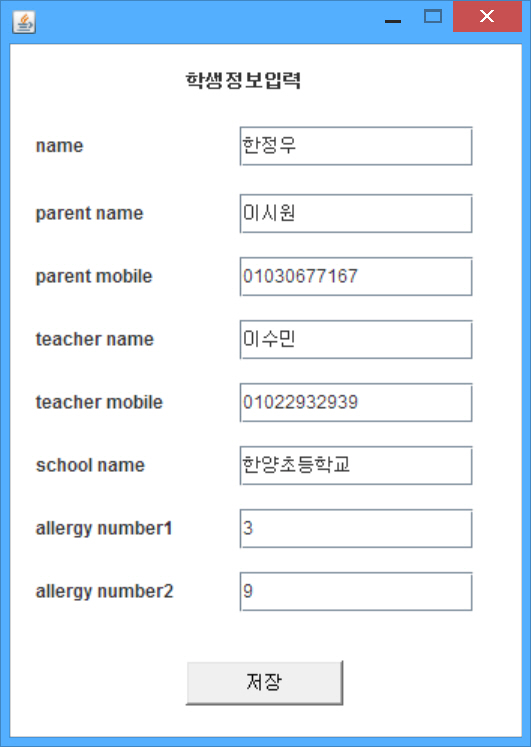
\includegraphics[width=0.4\textwidth]{usec9.jpg}
        \caption{}
        \label{fig1}
\end{figure}
~\\
user will see the registration window such as figure 18. The user write the information into the compartment such as id, pw, name, mobile, phone. and if user click "sign up" button , information should go into the table $teacher_info$ of database $allergorithm$. and window of join should shut down. This is possible because the login information of the user now been stored in the database. when the user enter id and password in the text field and click on the "log-in" button, id and password value of the user shall be checked whether valid. if the value of id and password is valid, home panel pop up.
And then, you can write the student’s information about name/parent name/parent mobile/teacher name/teacher mobile/ school name/ allergy number1/ allergy number2. The textbox parent mobile and teacher mobile are very important. Because we programmed that SMS is sent to that phone number. 
If you click the store button at the bottom side. , the program takes each values and pass the values to the databases. Let’s see the result.
~\\
\begin{figure}[!h]
        \centering
        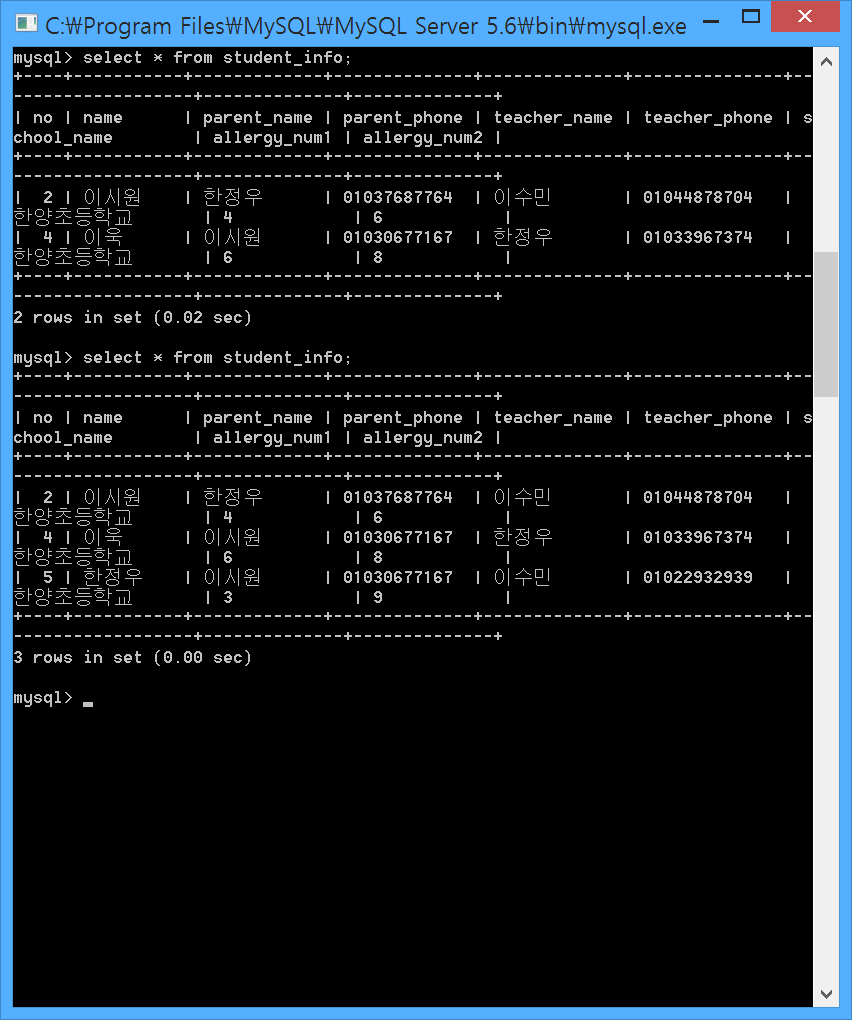
\includegraphics[width=0.5\textwidth, height=0.5\textheight]{usec10.jpg}
        \caption{}
        \label{fig1}
\end{figure}
~\\
You can see the student’s information is stored in the database in figure 32. After you write the student registeration, this information is enrolled in the $student_info$ table. As you can see, student Han Jeong Woo is added. This information means that student Han Jeong Woo whose parent's name is Lee Si Won and the Parent number is 01030677167 has allergic reaction about number 3 and 9 which are buckwheat and shrimp. The program search and match the $allergy_num1$ column with the $month_menu$ table.
~\\
\newpage
\begin{figure}[!h]
        \centering
        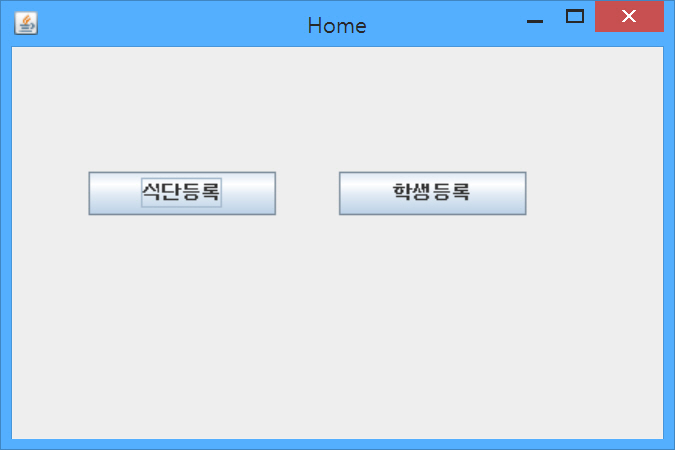
\includegraphics[width=0.4\textwidth]{usec11.jpg}
        \caption{}
        \label{fig1}
\end{figure}
~\\
And in this step, If you click the left button that can register food menu, This figure pops up.
The above table is illustrating a process after login. when user presses a register diet button on the Home panel, a panel pops up where you can enter the diets of the day. when the user has pressed the enter button, the value stored in the text field are stored in the table named $month_menu$. and when user presses a register student button on the Home panel, a panel pops up where you can enter information of the student. when the user has pressed the enter button, the value stored in the text field are stored in the table named $student_info$.
You can register the date from 1 to 31.
~\\
\begin{figure}[!h]
        \centering
        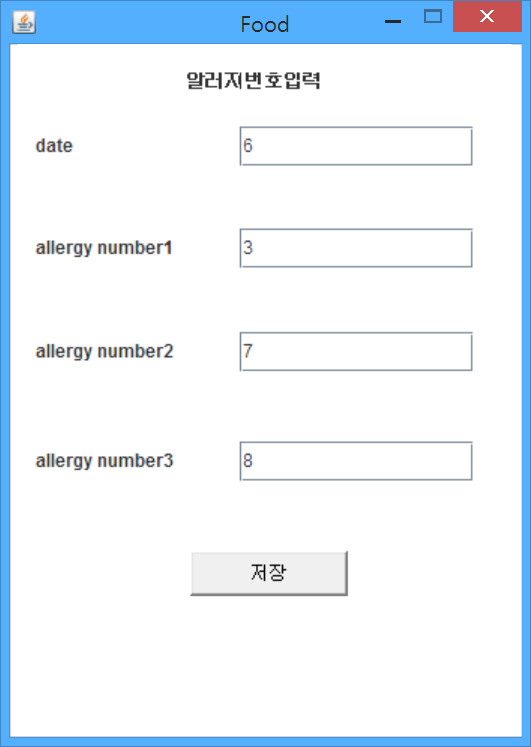
\includegraphics[width=0.4\textwidth]{usec12.jpg}
        \caption{}
        \label{fig1}
\end{figure}
~\\
The following table is a diet registration panel. user need to enter information, date, allergy number 1, allergy number 2, allergy number 3, a total of four. the date is one essential information you need to enter. The other three spaces are not essential. Because there is no allergens meals day. Press the Enter button and enter the information so that the information you enter in the text field are stored in the database. So each tuple is numbered  each time when the user enters the individual information, there isn't tha way that tuple is overlapped.
~\\
\begin{figure}[!h]
        \centering
        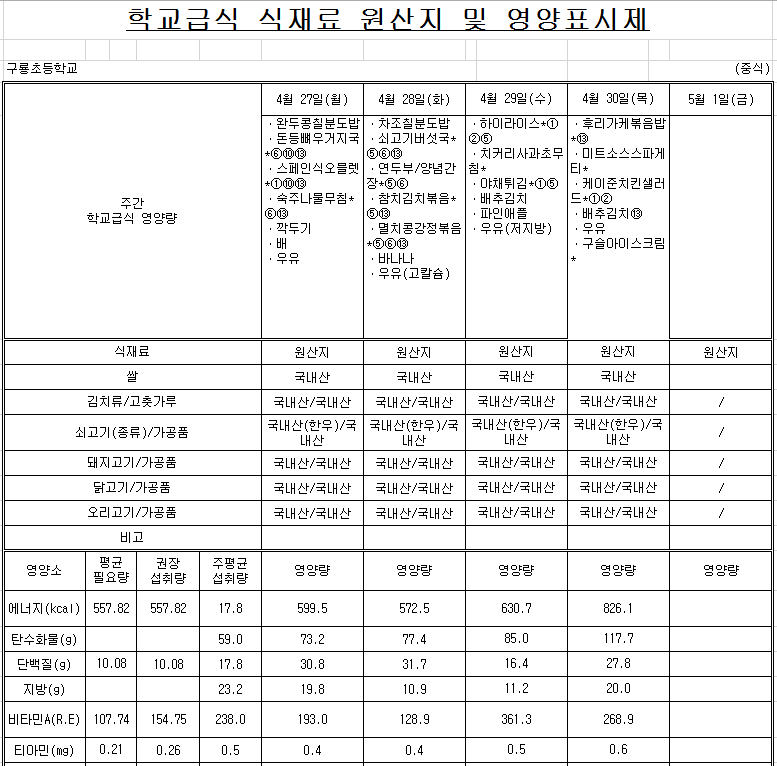
\includegraphics[width=0.5\textwidth, height=0.5\textheight]{usec13.jpg}
        \caption{}
        \label{fig1}
\end{figure}
~\\
If you want to register 4.27 food menu, you just write 27 at the date textbox, 1 at the allergy number1, 6 at the allergy number2, 10 at the allergy number3. Then you click the store button at the bottom side, the program takes each values and pass the values to the databases. Let’s see the result.
~\\
\newpage
\begin{figure}[!h]
        \centering
        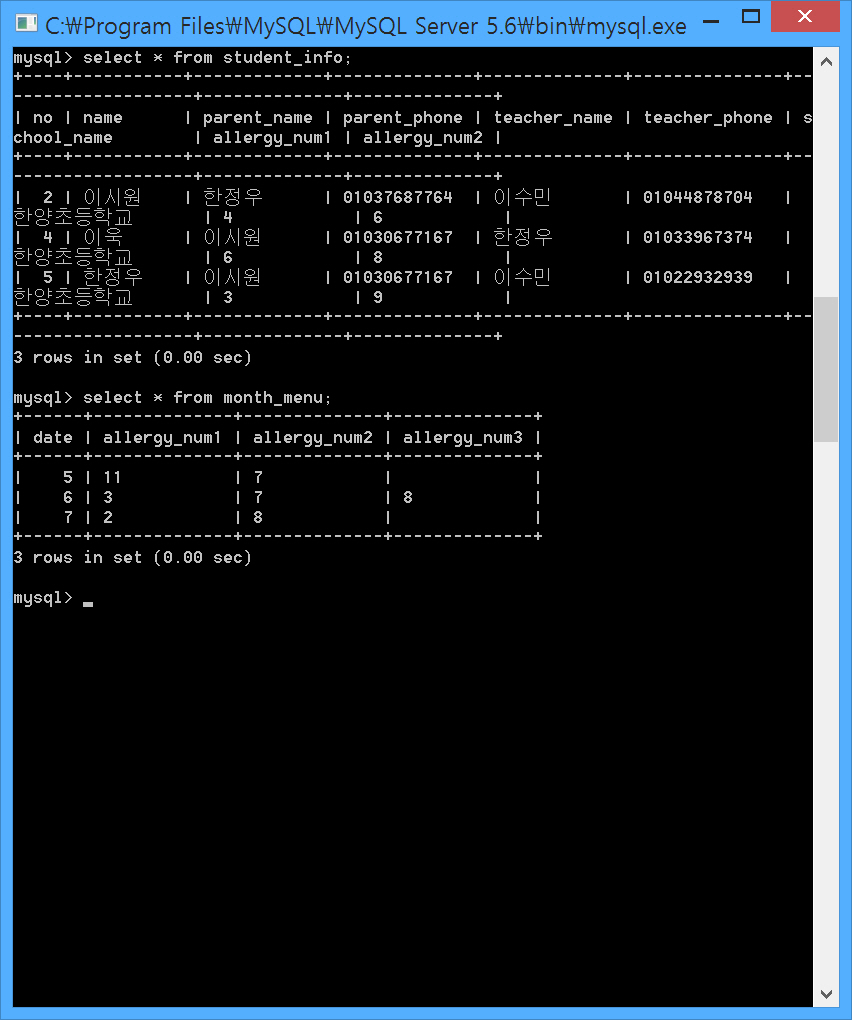
\includegraphics[width=0.5\textwidth, height=0.4\textheight]{usec14.jpg}
        \caption{}
        \label{fig1}
\end{figure}
~\\
After the writing, If you execute the com java file, the program pass the information to the SMS part. This means the database which contain the date, allergy number 1,2,3. All school have the same allergy number for the same food. Here are the example.  1.eggs 2.milk 3.buckwheat 4.peanuts 5.beans 6.wheat 7.mackerel 8.crab 9.shrimp 10.pork 11.peach 12.tomato. So the database information means that mackerel, peach are provided at date 5. By the same principle buckwheat, mackerel,crab are provided at date 6.
~\\
\newpage
\begin{figure}[!h]
        \centering
        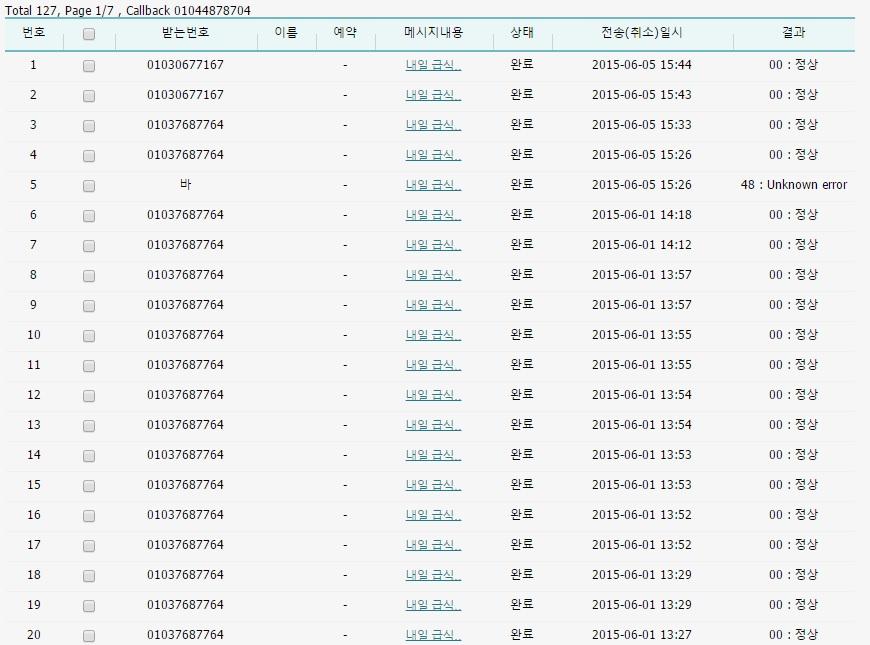
\includegraphics[width=0.5\textwidth, height=0.4\textheight]{usec15.jpg}
        \caption{}
        \label{fig1}
\end{figure}
~\\
the figure 37 is our testing history. If we click the button in the program, it relates the code with web site who can send the message. Before the testing, We charge the  sending message. It imposed us 40won for each message. The number 5 message get error because receiver's number are wrong. If the state is success, We can get a message.
~\\
\newpage
\begin{figure}[!h]
        \centering
        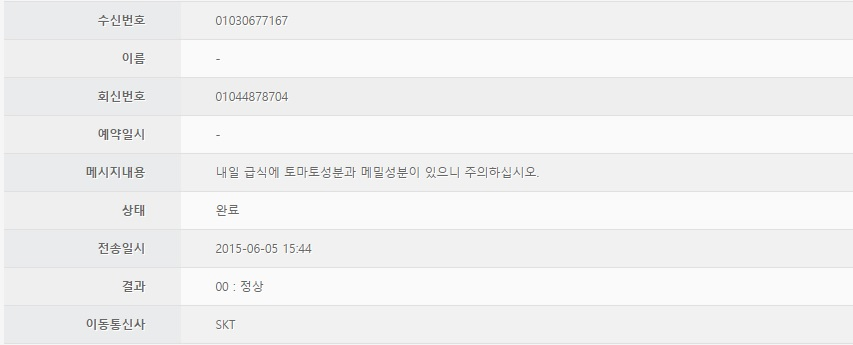
\includegraphics[width=0.5\textwidth, height=0.4\textheight]{usec16.jpg}
        \caption{}
        \label{fig1}
\end{figure}
~\\
~\\
\begin{figure}[!h]
        \centering
        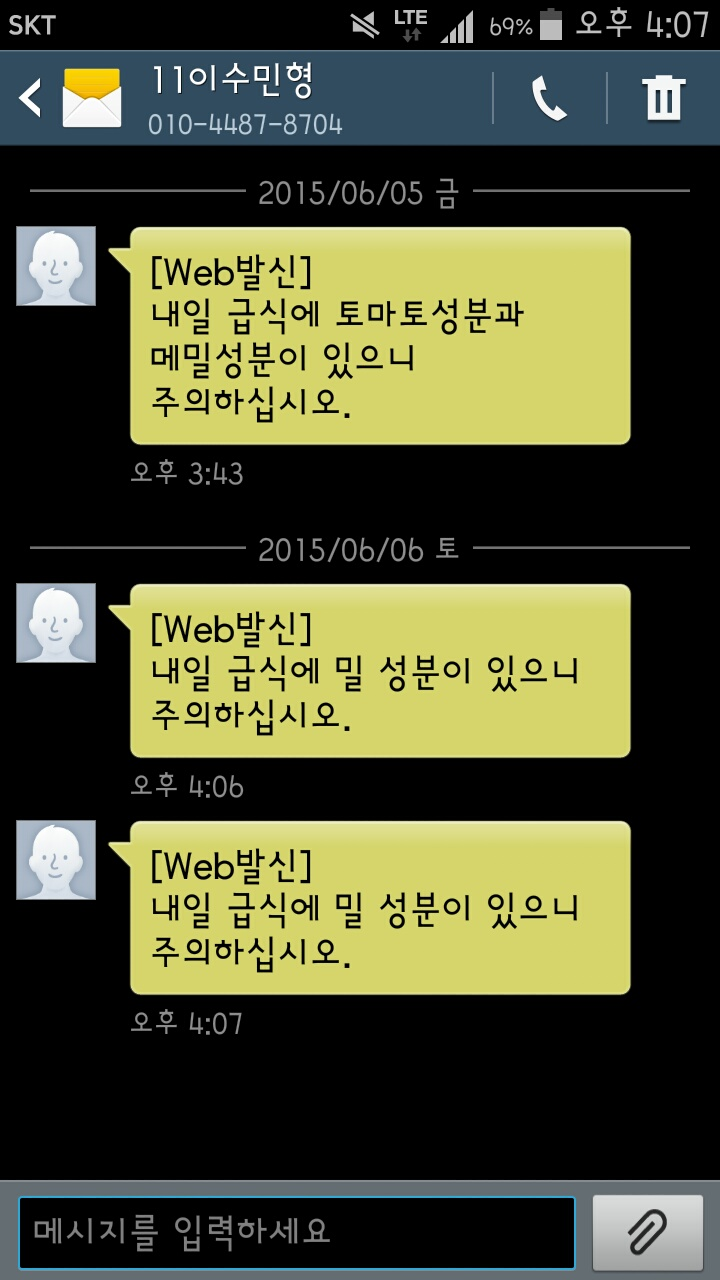
\includegraphics[width=0.4\textwidth, height=0.4\textheight]{usec17.jpg}
        \caption{}
        \label{fig1}
\end{figure}
~\\
~\\
\begin{figure}[!h]
        \centering
        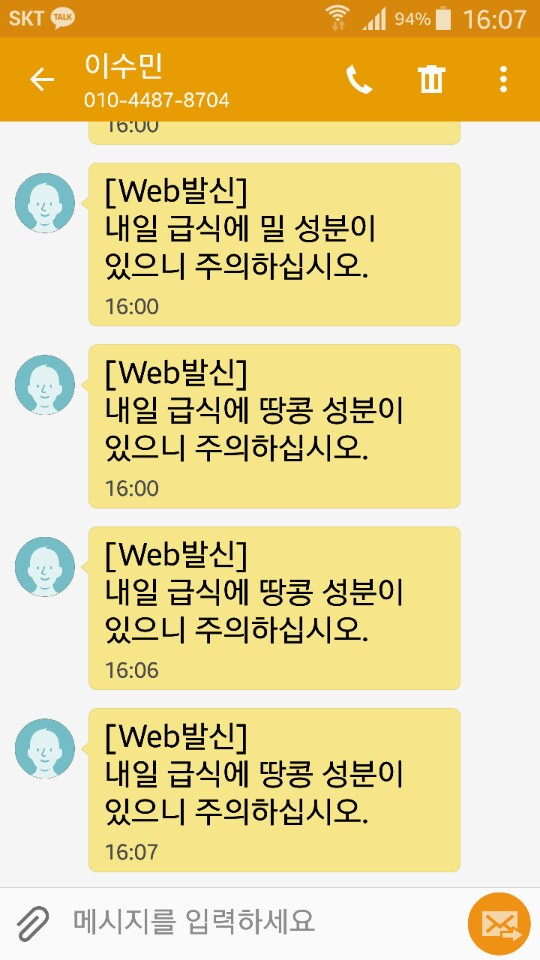
\includegraphics[width=0.4\textwidth]{usec18.jpg}
        \caption{}
        \label{fig1}
\end{figure}
~\\
These are the result of our program. We signed up the foods for each numbers. These two students both have wheat allergy. The message sender is set Lee Su Min. If you use this program actually, We can reset the sender's number. The program has the information of students and menu. Additionally it can take the information by the number and express the result. If you write the allergy number 6,12, the message will inform that tomorrow's menu is wheat and tomato.
~\\
}
\begin{thebibliography}{1}
\bibitem{IEEEhowto:kopka}
H.~Kopka and P.~W. Daly, \emph{A Guide to \LaTeX}, 3rd~ed.\hskip 1em plus
  0.5em minus 0.4em\relax Harlow, England: Addison-Wesley, 1999.

\end{thebibliography}

\end{document}

